
\chapter{Disparity from Truck Data}
\label{chap:Res}
In the previous section, the third dimension of a point is detected using corresponding features detected from multiple images using a technique known as thr Structure From Motion. In this section the third dimension is detected using sensor data available from the truck. This data includes total number of rotations from the optical shaft encoder and the steering Angle from the potentiometer. 

\section{Coordinate Information from Sensor Values}

The optical shaft encoder in the truck operates by translating the rotation of the shaft into light interruptions in the form of electrical pulses. The device gives output value as the total rotations performed by the wheel.

If the rotation is assumed as \(\omega\), then the distance travelled is given by \[ d = \omega \times l = 2\times \pi \times r \] where $l$ is the circumference of the truck wheel and $r$ is the radius of the truck wheel. This result is the distance travelled by the truck.

The potentiometer in the truck returns value that is propotional to the steering angle of the truck and if $x$ and $y$ are the plane coordinates of the current position of the truck then, \[ y=d \times cos\theta, x=d \times sin\theta, \] 

where $\theta$ is the steering angle. At this point the z position of the truck is assumed to be zero. In future, if a gyro sensor is added to the system then the third coordinate of the point can be directly detected from the sensor.

The coordinates are stored as \( \delta x , \delta y , \delta z \) where $\delta$ represents the change in the value. The incremental changes are added together to obtain the total change in the x and y from the initial position.

\section{Fundamental Matrix from Sensor Values}
	The points detected in the previous section are in 3D space. To convert them into the image plane.
	\( x'=K \times x \) , where x is the current point in the 3D space and $x'$ is the point in the image plane . The transformation between the $x$ and $x'$ in the world plane is given by 
	\[
  T=
  \left[ {\begin{array}{ccc}
   cos \theta & sin \theta & tx\\
   -sin \theta & cos \theta & ty \\
   0 & 0 & 1 \\
  \end{array} } \right]
\]
Here $tx$ and $ty$ are the \( \delta x , \delta y \) and \(\theta\) is the change in the angle from the previous position. This transformation matrix in the image plane is given as \( P'=K P \) in \cite{hartley2003multiple}.

 For example if the first point is taken at the origin then it can be represented as \[ P =K[I | 0] \] in the image plane. Where $K$ is the camera matrix, the second point can be represented as \[ P' =K [R | t] \] and if the Psuedo inverse \({P}^+\) is given as 
\[
  {P}^+=
  \left[ {\begin{array}{c}
   {K}^{-1} \\
   0  \\
   \end{array} } \right]
\] 
and the camera center C is given as 
\[
  C=
  \left[ {\begin{array}{c}
   0\\
   1\\
   \end{array} } \right]
\]

then the Fundamental Matrix is given by 
\[F = [P'C]P'P^{+}\]

 From $F$ the essential matrix can be computed and from the triangulation of the points in the plane, an estimate of the $z$ coordinate can be determined as shown in \cite{hartley2003multiple}.

\paragraph{ Calculate xyz from  Sensor Values}
\paragraph{Description}
This function uses the truck sensor values to calculate the x and y coordinate.
\paragraph{Synopsis:}
\begin{lstlisting}
void calcualtexyz(float Encoder_data, 
				  float theta, 
				  coordinates &xyz_Data );
\end{lstlisting}

\paragraph{ Calculate Fundamental Matrix from xyz}
\paragraph{Description}
This function uses x, y coordinates and the camera matrices to calculate the fundamental matrix .
\paragraph{Synopsis:}
\begin{lstlisting}
void CameraMatrixxyz(coordinates &xyz_Data, const Mat& K, 
					 const Mat& Kinv, const Mat& distcoeff,
					 Matx34d& P, Matx34d& P1, vector<CloudPoint> &outCloud); 
\end{lstlisting}
   \begin{figure}[h]
    \centering
    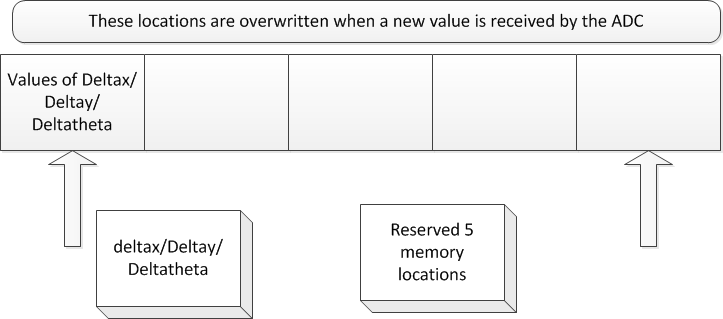
\includegraphics[width=14cm,height=14cm,keepaspectratio]{Pictures/deltax}
    \caption{Storage $\delta$x}
    \label{fig:deltax}
	\end{figure}

\begin{figure}[h]
    \centering
    \includegraphics[width=15cm,height=15cm,keepaspectratio]{Pictures/Truck}
    \caption{Transformation}
    \label{fig:truck}
  \end{figure}

After calculating the camera matrices, functions from the previous section can be used to calculate the Z coordinate. This algorithm is known as triangulations.
